\section{Revisione del punto di vista degli sviluppatori}
\subsection{Risultati Preliminari}

Lo studio preliminare è stato condotto su 500 partecipanti.

Il numero di partecipanti che ha risposto correttamente alla domanda filtro è 188, rappresentando il 37,8\% della popolazione, come raffigurato in Figura \ref{fig:pre_filter}.

\begin{figure}[h!]
    \centering
    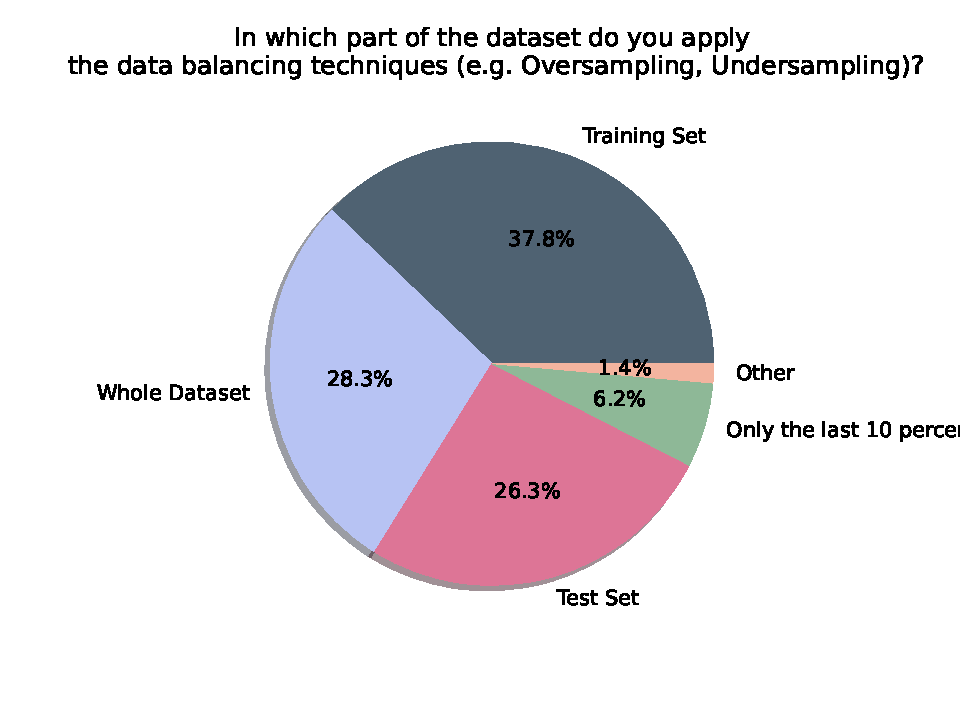
\includegraphics[width=0.8\textwidth]{Figure/Results/SurveyResults/prescreening/prescreening_filter_pie.pdf}
    \caption{Risposte alla domanda filtro del questionario di preselezione}
    \label{fig:pre_filter}
\end{figure}

Infine, applicando i filtri sulle competenze generali del settore e sulle competenze specifiche di intelligenza artificiale, sono stati esclusi 75 partecipanti.
Il numero di partecipanti che è stato accettato per condurre l'esperimento è 113.
La suddivisione dei partecipanti nei tre gruppi sperimentali è stata riportata in Tabella \ref{tab:design_experiment_results}.
\begin{table}[h]
    \centering
    \begin{tabular}{|c|c|c|}
        \hline
        \textbf{Partecipanti} & \textbf{Istanze di Ai Technical Debt}  & \textbf{Numero}\\
        \hline
        Gruppo 1 & Gruppo A+B & 37 \\
        Gruppo 2 & Gruppo B+C & 38\\
        Gruppo 3 & Gruppo A+C & 38\\
        \hline
    \end{tabular}
    \caption{Suddivisione dei partecipanti per gruppi di Ai Technical Debt}
    \label{tab:design_experiment_results}
\end{table}

Tuttavia non tutti i partecipanti hanno deciso di continuare l'esperimento, abbandonando lo studio durante la conduzione dell'esperimento.

Il numero di partecipanti invece a cui è stato sottoposto il questionario finale con successo è 54.

Da ogni risposta sottomessa da ogni partecipante sono state estratte poi i due gruppi sperimentali di riferimento ed è stato possibile quindi ottenere, per ogni gruppo di istanza di AI Technical Debt ottenere il numero di risposte riportato in Tabella \ref{tab:group_exp_results}.


\begin{table}[h]
    \centering
    \begin{tabular}{|c|p{6.5cm}|c|}
    \hline
        \textbf{Gruppi} & \textbf{Istanze AITD} & \textbf{Numero di Risposte}  \\
        \hline
        A &  Glue Code, Multiple Language Smell, Undeclared Consumers & 38 \\
        \hline
        B &  Pipeline Jungles, Correction Cascades, Scattered Use of ML
Libraries & 36 \\
        \hline
        C &  Jumbled Model Architecture, Unwanted Debugging Code,
Deep God File & 34 \\
\hline
    \end{tabular}
    \caption{Numero di risposte per ogni gruppo sperimentale di AI Technical Debt}
    \label{tab:group_exp_results}
\end{table}
%aggiungere la tabella delle risposte con i valori per ogni gruppo.

La Figura \ref{fig:general_skills} e la Figura \ref{fig:ai_skills} mostrano la distribuzione del livello di competenza dei partecipanti su aspetti generali della programmazione, software engineering e intelligenza artificiale, per poi approfondire sulle pratiche di intelligenza artificiale.
In particolare, è possibile notare come i partecipanti in media hanno una discreta conoscenza sulle tre discipline generali definite, riportando nella distribuzione una leggera variazione della mediana, dove le mediane con il valore più alto sono rispettivamente sulla distribuzione delle competenze di programmazione e sulla distribuzione delle competenze di intelligenza artificiale. Questo dato riporta come informazione che il livello di competenza dei partecipanti, anche se leggermente, è maggiormente orientato sulle conoscenze di intelligenza artificiale che quelle di ingegneria del software.
Situazione analoga per le competenze relative alle pratiche di intelligenza artificiale, dove ritroviamo un leggero aumento della mediana a $4/5$ per le attività di data preparation e utilizzo del codice delle librerie di Machine learning.

\begin{figure}[h!]
    \centering
    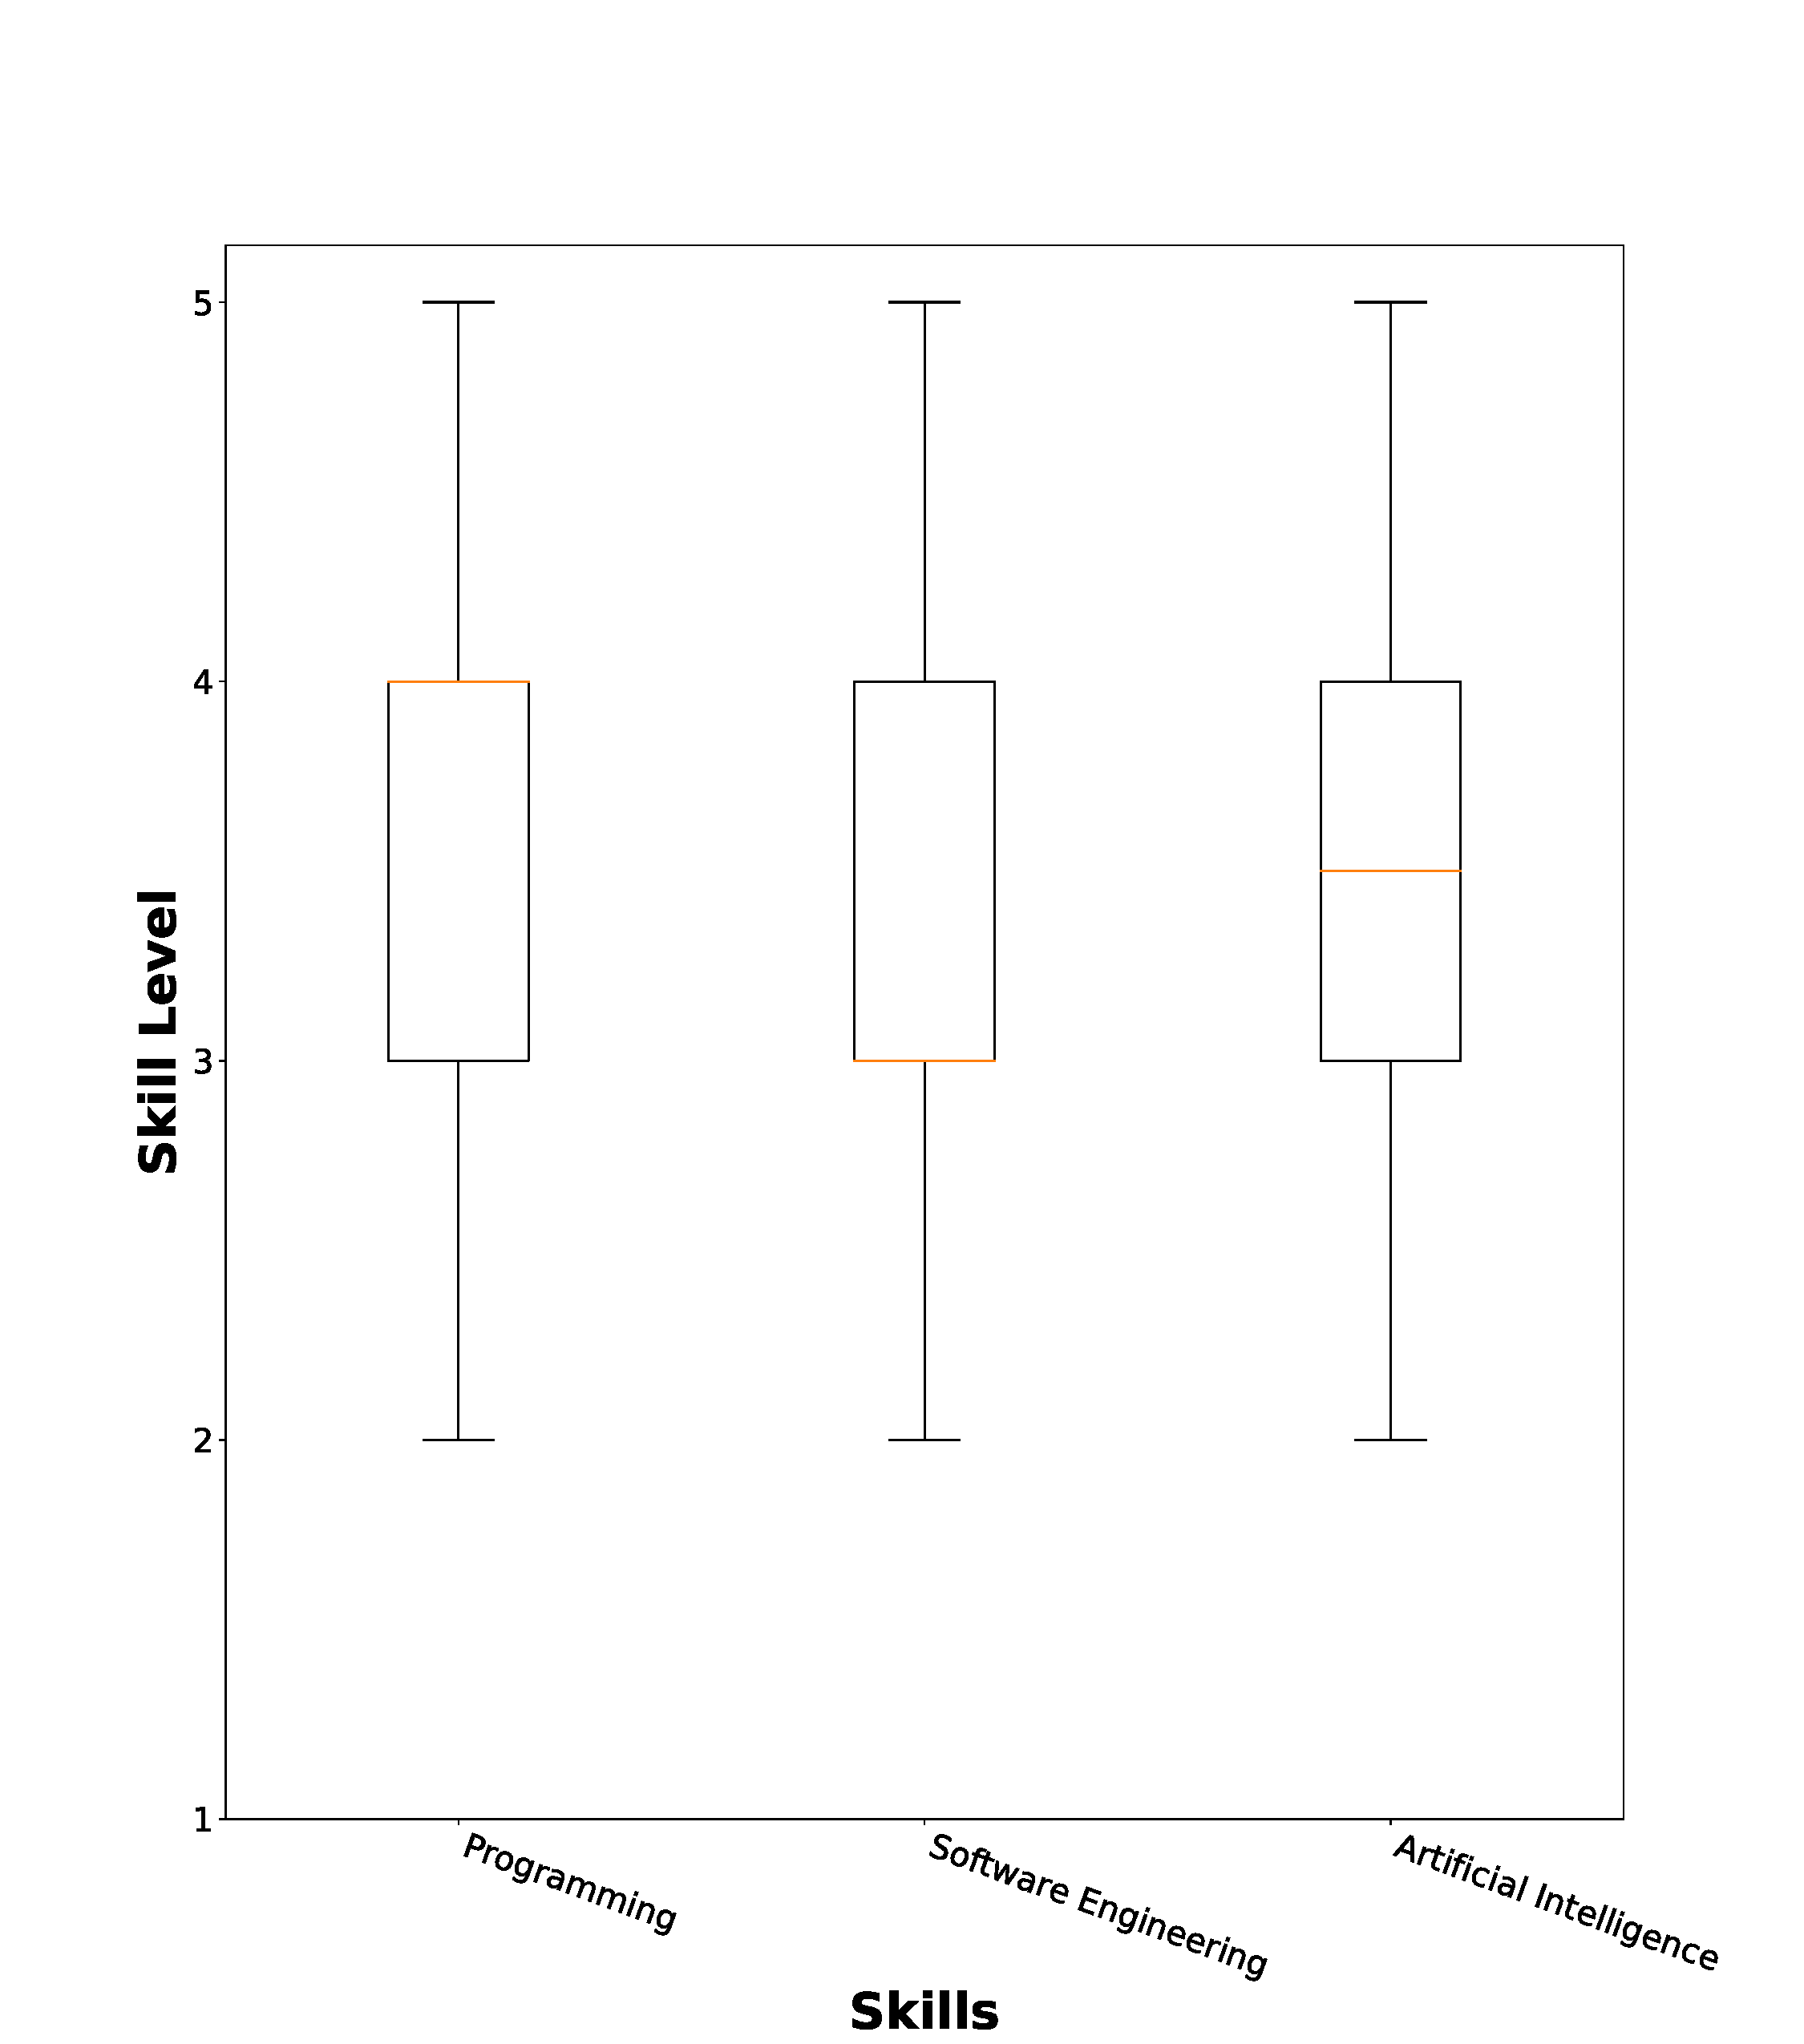
\includegraphics[width=\textwidth]{Figure/Results/SurveyResults/prescreening/def_skills_participant.pdf}
    \caption{Competenze generali dei partecipanti inclusi nel questionario}
    \label{fig:general_skills}
\end{figure}

\begin{figure}[h!]
    \centering
    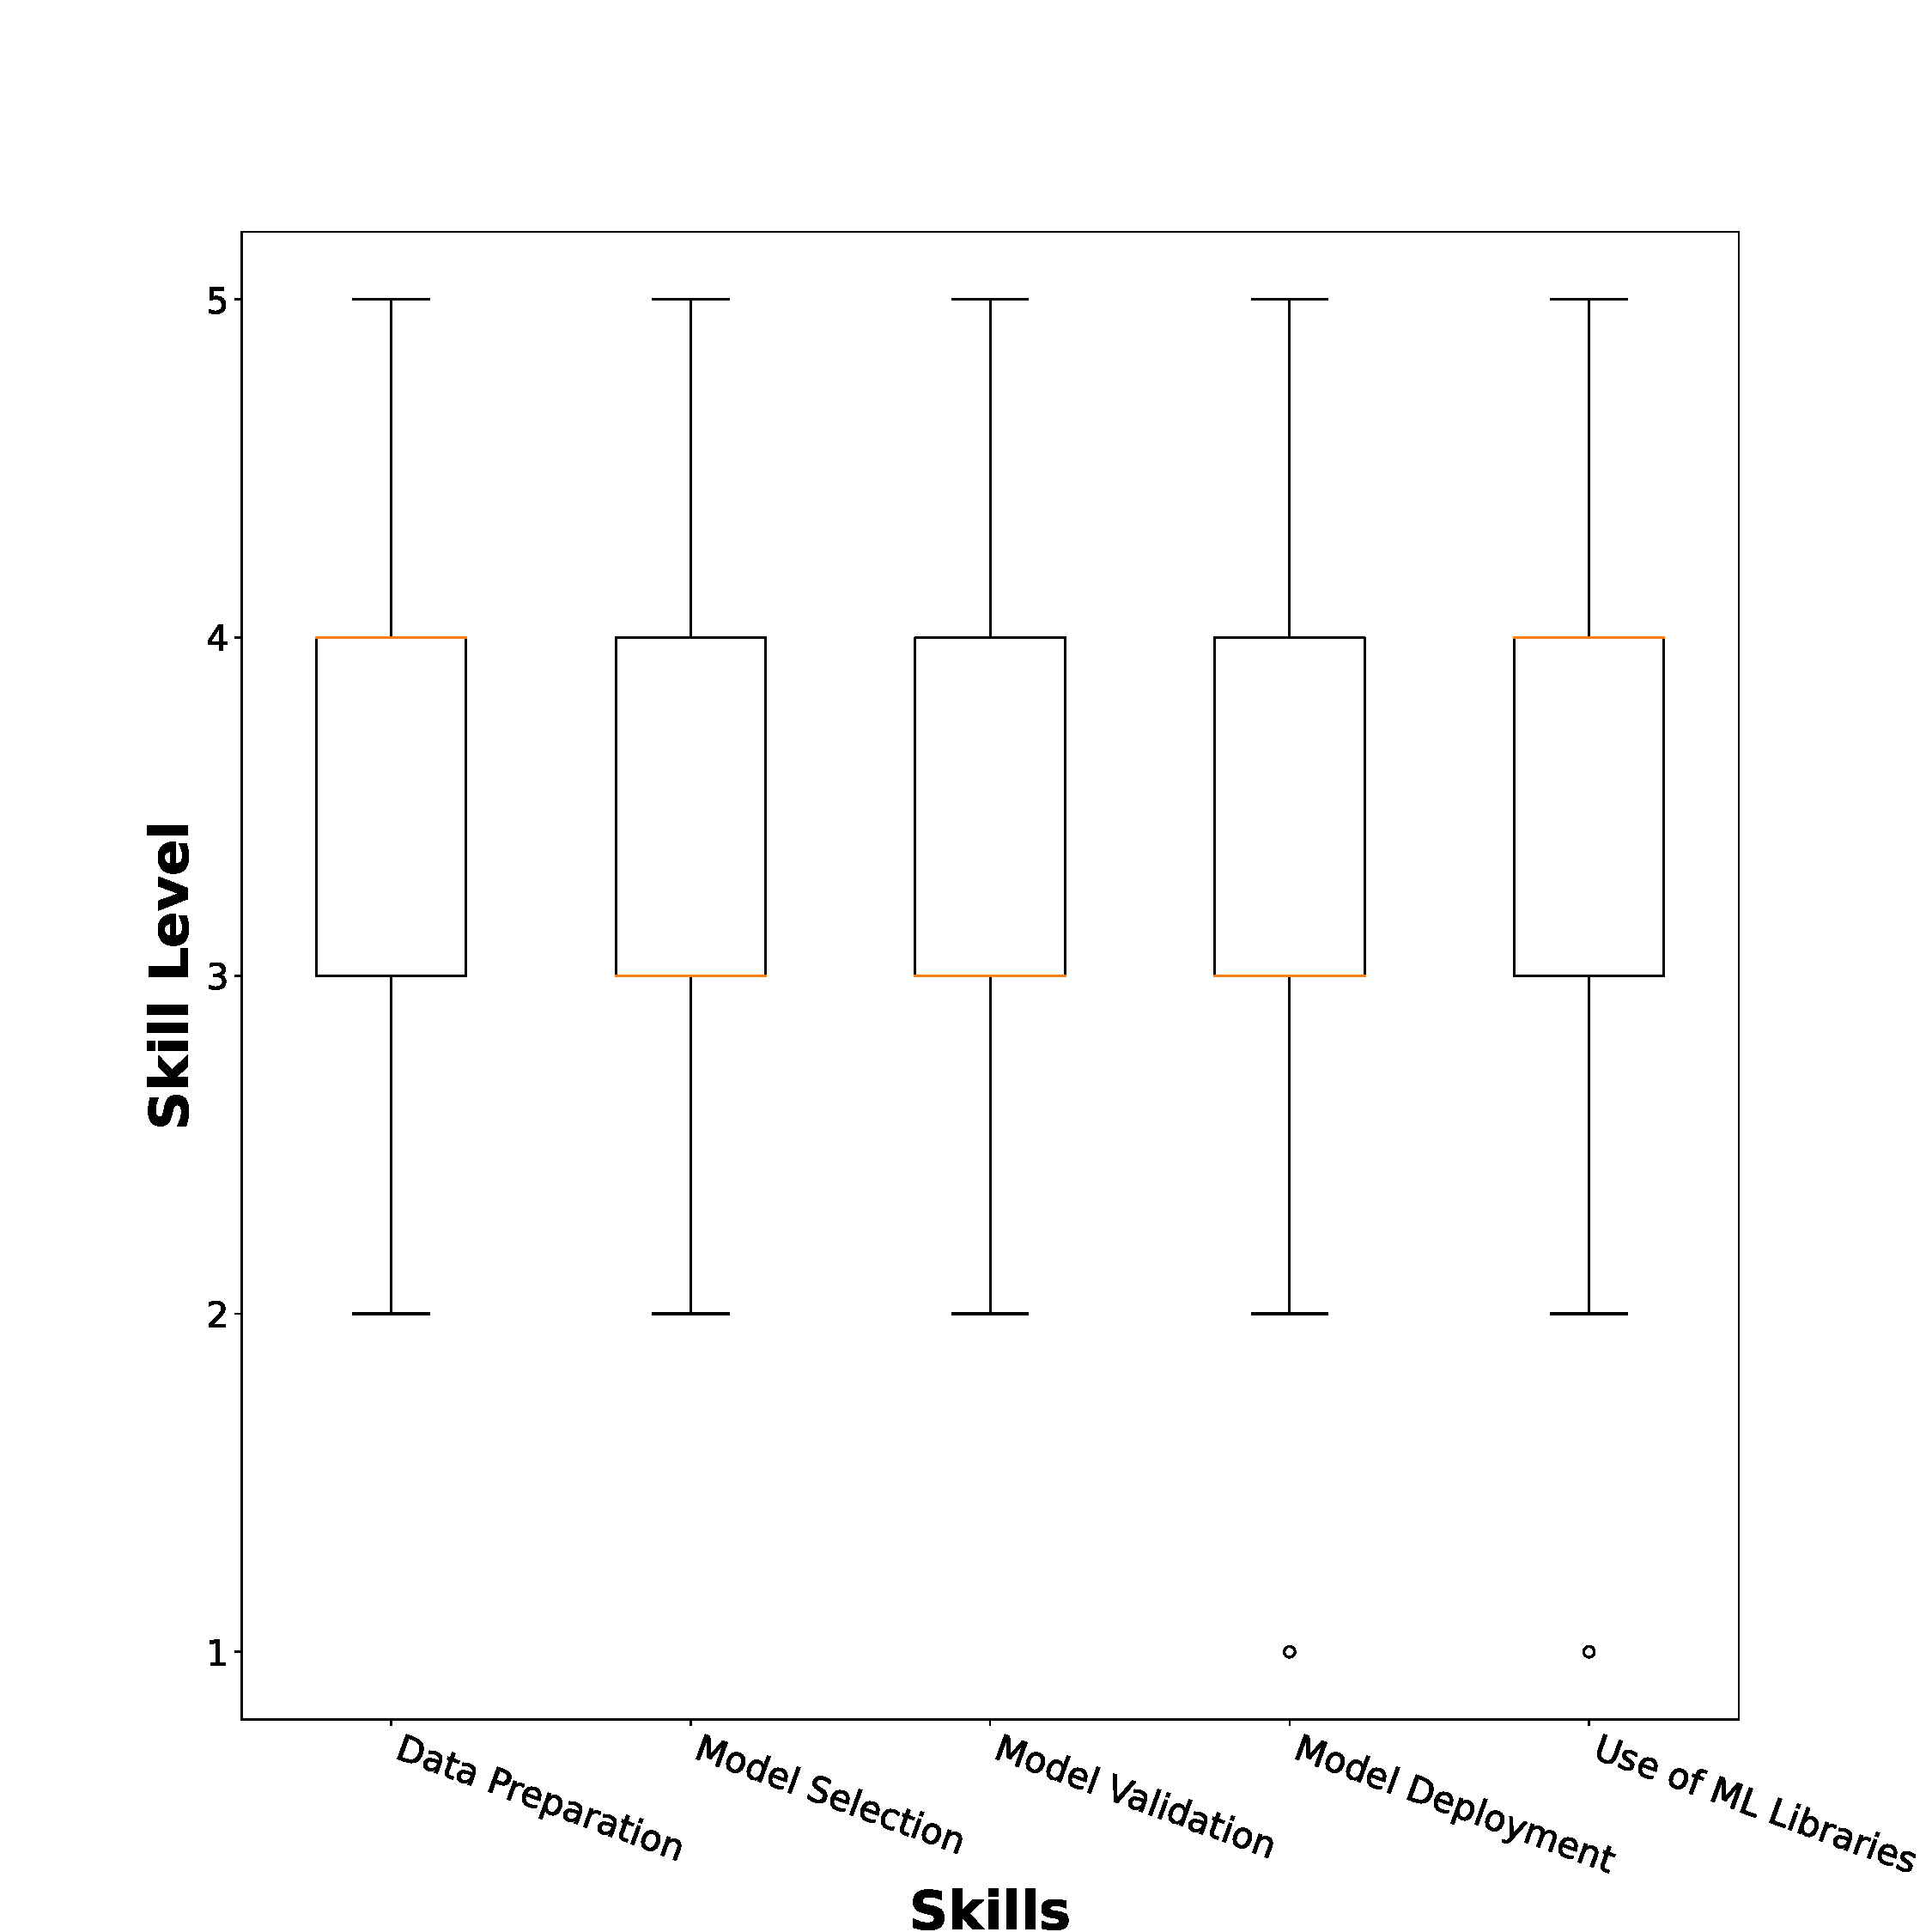
\includegraphics[width=\textwidth]{Figure/Results/SurveyResults/prescreening/def_ai_skills_participant.pdf}
    \caption{Competenze di intelligenza artificiale dei partecipanti inclusi nel questionario}
    \label{fig:ai_skills}
\end{figure}


\subsection{RQ2.1: Quali sono le tipologie di code debt e architectural debt più frequenti secondo la percezione degli sviluppatori AI?}

Secondo le analisi effettuate, i risultati si trovano in accordo con quanto ritrovato nella letteratura.
Considerando gli AI-Technical Debt che sono relativi all'architettura e al codice del sistema, \textit{Pipeline Jungle} e \textit{Glue Code} sono i più diffusi secondo la percezione degli sviluppatori.
La Tabella \ref{tab:freq_index} rappresenta la distribuzione dei valori del livello di frequenza che gli sviluppatori hanno dato per ogni istanza di AI Technical Debt.
In totale, solo 4 particolari istanze di AI Technical Debt vengono percepite da parte degli sviluppatori nel poter avere un'alta frequenza: \textit{Pipeline Jungle}, \textit{Glue Code}, \textit{Jumbled Model Architecture}, \textit{Unwanted Debugging Code}.
Tuttavia, la maggior parte degli sviluppatori ritiene un discreto tasso di frequenza solo per due delle istanze definite:\textit{Pipeline Jungle} e \textit{Glue Code}.

\begin{table}[h]
    \footnotesize
    \centering
    \begin{tabular}{|l|c|c|c|c|}
    \hline
    \textbf{AI Technical Debt Instance} & \textbf{Mediana} & \textbf{Media} & \textbf{Dev. Std.} & \textbf{Moda} \\
    \hline
    Glue Code & \textbf{3.0} & 2.45 & 1.11 & \textbf{3.0} \\
    Multiple Language Smell & 2.0 & 2.05 & 1.11 & 1.0 \\
    Undeclared Consumers & 2.0 & 1.97 & 1.08 & 1.0 \\
    Pipeline Jungle & \textbf{2.5} &\textbf{2.69} & 1.17 & 2.0 \\
    Correction Cascades & 2.0 & 2.44 & 1.03 & 2.0 \\
    Scattered Use of ML Libraries & 2.0 & 2.17 & 1.23 & 1.0 \\
    Jumbled Model Architecture & 2.0 & \textbf{2.53} & 1.02 & 2.0 \\
    Unwanted Debugging Code & 2.0 & 2.5 & 1.24 & 2.0 \\
    Deep God File & 2.0 & 2.18 & 1.03 & 2.0 \\
    \hline
    \end{tabular}
    \caption{Distribuzione della diffusione di AI Technical Debt secondo la percezione degli sviluppatori}
    \label{tab:freq_index}
\end{table}

\subsection{RQ2.2: Quali sono le tipologie di code debt e architectural debt più problematiche secondo la percezione degli sviluppatori AI?}

Gli sviluppatori hanno riportato tre particolari istanze di AI Technical Debt come problematiche all'interno del sistema. 
\textit{Undeclared Consumers}, la quale presenta una moda di severità pari al massimo nella distribuzione dei dati, è considerato per gli sviluppatori il più problematico per i sistemi AI,come illustrato in Tabella \ref{tab:sev_index}.
Le motivazioni raccolte dai partecipanti sono riguardanti l'aspetto di sicurezza, in quanto la presenza di questa particolare istanza di AI Technical Debt può essere sfruttata al fine di comprendere il funzionamento del modello di intelligenza artificiale e effettuare attacchi malevoli.
In particolare, un partecipante ha risposto spiegando che si trova molto spesso a lavorare con dati sensibili e questo può essere una grave falla di sicurezza utilizzabile per diffondere quei dati.
Inoltre la percezione degli sviluppatori ha riscontrato un'alta severità per le istanze di \textit{Pipeline Jungle} e \textit{Jumbled Model Architecture}.
Entrambe le istanze causano una crescita incontrollata del sistema, riportando gravi problematiche di complessità e manutenibilità.
In particolare, un partecipante, in considerazione della presenza di un istanza di \textit{Jumbled Model Architecture} ha risposto che la problematica nasce quando si ha a che fare con un sistema di grandi dimensioni, dove uno sviluppatore in fase di manutenzione del sistema deve affrontare una mancanza di chiarezza e di riconoscibilità delle componenti.

\begin{table}[h]
    \footnotesize
    \centering
    \begin{tabular}{|l|c|c|c|c|}
    \hline
    \textbf{AI Technical Debt Instance} & \textbf{Mediana} & \textbf{Media} & \textbf{Dev. Std.} & \textbf{Moda} \\
    \hline
    Glue Code & 3.0 & 2.92 & 1.32 & 2.0 \\
    Multiple Language Smell & 3.0 & 3.0 & 1.47 & 4.0 \\
    Undeclared Consumers & \textbf{4.0} & \textbf{3.73} & 1.32 & \textbf{5.0} \\
    Pipeline Jungle & \textbf{4.0} & 3.47 & 1.13 & 4.0 \\
    Correction Cascades & 3.0 & 3.22 & 1.22 & 4.0 \\
    Scattered Use of ML Libraries & 3.0 & 3.02 & 1.38 & 4.0 \\
    Jumbled Model Architecture & \textbf{4.0} & 3.47 & 1.0 & 4.0 \\
    Unwanted Debugging Code & 2.0 & 2.32 & 1.22 & 1.0 \\
    Deep God File & 3.0 & 3.11 & 1.45 & 2.0 \\
    \hline
    \end{tabular}
    \caption{Indice di severità delle diverse istanze di AI Technical Debt secondo la percezione degli sviluppatori.}
    \label{tab:sev_index}
\end{table}

In aggiunta lo sforzo di identificazione e lo sforzo di mitigazione delle istanze di AI Technical Debt percepito dagli sviluppatori è riportato rispettivamente in Tabella \ref{tab:id_effort_index} e in Tabella \ref{tab:ref_effort_index}.
Anche sotto questo aspetto, gli sviluppatori ritengono che l'identificazione e la mitigazione per le istanze di \textit{Undeclared Consumers, Pipeline Jungle} e \textit{Jumbled Model Architecture} richiede un'alto effort.
Essendo istanze di AI Technical Debt che interferiscono sul sistema a livello architetturale, queste istanze portano un calo degli attributi di qualità su tutta l'architettura del sistema. Questa granularità così alta, a differenza dei dati e del codice, comporta ad aumentare la difficoltà di identificare e mitigare un problema presente.
Inoltre, in caso di presenza di istanze come \textit{Correction Cascades} o \textit{Deep God File}, gli sviluppatori ritengono che la mitigazione di queste particolari istanze possa richiedere un'alto effort.

\begin{table}[h!]
    \footnotesize
    \centering
    \begin{tabular}{|l|c|c|c|c|}
    \hline
    \textbf{AI Technical Debt Instance} & \textbf{Mediana} & \textbf{Media} & \textbf{Dev. Std.} & \textbf{Moda} \\
    \hline
    Glue Code & 3.0 & 2.92 & 1.32 & 2.0 \\
    Multiple Language Smell & 3.0 & 3.0 & 1.47 & 4.0 \\
    Undeclared Consumers & \textbf{4.0} & \textbf{3.74} & 1.33 & \textbf{5.0} \\
    Pipeline Jungle & \textbf{4.0} & 3.47 & 1.13 & 4.0 \\
    Correction Cascades & 3.0 & 3.22 & 1.22 & 4.0 \\
    Scattered Use of ML Libraries & 3.0 & 3.03 & 1.38 & 4.0 \\
    Jumbled Model Architecture & \textbf{4.0} & 3.47 & 1.02 & 4.0 \\
    Unwanted Debugging Code & 2.0 & 2.32 & 1.22 & 1.0 \\
    Deep God File & 3.0 & 3.12 & 1.45 & 2.0 \\
    \hline
    \end{tabular}
    \caption{Sforzo di identificazione delle diverse istanze di AI Technical Debt secondo la percezione degli sviluppatori.}
    \label{tab:id_effort_index}
\end{table}

\begin{table}[h!]
    \footnotesize
    \centering
    \begin{tabular}{|l|c|c|c|c|}
    \hline
    \textbf{AI Technical Debt Instance} & \textbf{Mediana} & \textbf{Media} & \textbf{Dev. Std.} & \textbf{Moda} \\
    \hline
    Glue Code & 3.0 & 2.95 & 1.23 & 2.0 \\
    Multiple Language Smell & \textbf{4.0} & 3.24 & 1.57 & 4.0 \\
    Undeclared Consumers & \textbf{4.0} & 3.53 & 1.29 & 4.0 \\
    Pipeline Jungle & \textbf{4.0} & 3.33 & 1.17 & 4.0 \\
    Correction Cascades & \textbf{4.0} & 3.5 & 1.18 & 4.0 \\
    Scattered Use of ML Libraries & 3.0 & 3.0 & 1.41 & 2.0 \\
    Jumbled Model Architecture & \textbf{4.0} & \textbf{3.82} & 1.03 & \textbf{5.0} \\
    Unwanted Debugging Code & 2.0 & 2.09 & 1.24 & 1.0 \\
    Deep God File & \textbf{4.0} & 3.71 & 1.19 & 4.0 \\
    \hline
    \end{tabular}
    \caption{Sforzo di mitigazione delle diverse istanze di AI Technical Debt secondo la percezione degli sviluppatori.}
    \label{tab:ref_effort_index}
\end{table}

\subsection{RQ2.3: Qual è l’impatto causato dai code debt e architectural debt secondo la percezione degli sviluppatori AI?}

La Tabella \ref{tab:impact_pt1} riporta i risultati delle analisi relative alle caratteristiche di qualità di impatto sulla altre componenti dei sistemi AI, sulla comprensibilità e sull'evoluzione.
Secondo il punto degli sviluppatori, l'impatto più alto sulle altri componenti del sistema è causato dalla presenza di \textit{Undeclared Consumers}, considerando che un libero accesso ai dati in output del modello, possa permettere ad applicazioni esterne e sconosciute di avere un impatto su tutte le componenti del sistema.

La comprensibilità del codice del software è, secondo il punto di vista degli sviluppatori, un aspetto di qualità che può essere influenzato da diverse istanze di AI Technical Debt. In particolare, dalle risposte riscontriamo \textit{Deep God File} con una mediana pari a 5, una media pari a 4.32 e una moda pari a 5. 
Inoltre, \textit{Pipeline Jungle}, \textit{Jumbled Model Architecture} e \textit{Correction Cascades} sono considerate molto problematiche e possibili cause di un calo della comprensibilità all'interno del sistema.

Molte delle istanze proposte agli sviluppatori sono ritenute invece come possibili minacce all'evoluzione del sistema.
In particolare, \textit{Deep God File}, la quale distribuzione delle risposte presenta una mediana pari a 4, una media pari a 4.21 e una moda pari a 5, è l'istanza di AI-Technical Debt più problematica per l'evoluzione di un sistema AI.
Inoltre, un'alta influenza sull'evoluzione del sistema è causata da \textit{Jumbled Model Architecture}, \textit{Correction Cascades}, \textit{Pipeline Jungle} e \textit{Multiple Language Smell}.



\begin{table}[h!]
    \footnotesize
    \centering
    \begin{tabular}{|l|c|c|c|c|c|}
    \hline
    Quality aspect & AI TechnicalDebt Instance & median & mean & std & mode \\
    \hline
\multirow{9}{*}{Impact}
& Glue Code & 3.0 & 2.89 & 1.27 & \textbf{4}   \\
& Multiple Language Smell & 3.0 & 3.03 & 1.42 & \textbf{4}   \\
& Undeclared Consumers & \textbf{4.0} & \textbf{3.76} & 1.24 & \textbf{4}   \\
& Pipeline Jungle & \textbf{4.0} & 3.44 & 1.08 &\textbf{4}   \\
& Correction Cascades & 3.0 & 3.31 & 1.24 & \textbf{4}   \\
& Scattered Use of ML Libraries & 2.5 & 2.64 & 1.33 & 1   \\
& Jumbled Model Architecture & 3.0 & 3.18 & 1.11 & \textbf{4}   \\
& Unwanted Debugging Code & 2.0 & 2.32 & 0.98 & 2   \\
& Deep God File & 3.0 & 3.29 & 1.31 & 3   \\
    \hline
\multirow{9}{*}{Understandability}
& Glue Code & 3.5 & 3.05 & 1.41 & 4  \\
& Multiple Language Smell & 4.0 & 3.32 & 1.68 & \textbf{5}  \\
& Undeclared Consumers & 3.0 & 3.03 & 1.22 & 4  \\
& Pipeline Jungle & 4.0 & 4.08 & 1.0 & \textbf{5}  \\
& Correction Cascades & 4.0 & 3.94 & 1.07 & 4  \\
& Scattered Use of ML Libraries & 3.0 & 3.14 & 1.44 & 4  \\
& Jumbled Model Architecture & 4.0 & 4.06 & 1.01 & 4  \\
& Unwanted Debugging Code & 2.0 & 2.24 & 1.13 & 2  \\
& Deep God File & \textbf{5.0} & \textbf{4.32} & 0.84 & \textbf{5}  \\
    \hline
\multirow{9}{*}{Evolution}
& Glue Code & 3.0 & 2.97 & 1.44 & 2 \\
& Multiple Language Smell & \textbf{4.0} & 3.61 & 1.5 & \textbf{5}  \\
& Undeclared Consumers & 3.0 & 3.08 & 1.46 & \textbf{5}  \\
& Pipeline Jungle & \textbf{4.0} & 3.86 & 1.15 & \textbf{5}  \\
& Correction Cascades & \textbf{4.0} & 3.75 & 1.13 & 4  \\
& Scattered Use of ML Libraries & 3.5 & 3.28 & 1.41 & 4  \\
& Jumbled Model Architecture & \textbf{4.0} & 3.94 & 1.18 & 4  \\
& Unwanted Debugging Code & 2.0 & 2.18 & 1.03 & 2  \\
& Deep God File & \textbf{4.0} & \textbf{4.21} & 0.95 & \textbf{5}  \\
    \hline
    \end{tabular}
    \caption{Effetti sull'impatto sulle componenti del sistema, comprensibilità e evoluzione delle diverse istanze di AI Technical Debt secondo la percezione degli sviluppatori.}
    \label{tab:impact_pt1}
\end{table}

La Tabella \ref{tab:impact_pt2} riporta i risultati delle analisi relative alle caratteristiche di qualità di perfomance, accoppiamento e manutenzione dei sistemi AI.
Secondo il punto degli sviluppatori, le performance del modello possono essere influenzate da diverse istanze di AI Technical Debt. La presenza di una \textit{Pipeline Jungle}, compromettendo il controllo e l'accessibilità alle fasi di gestione e di esecuzione della pipeline, inficiano sulle perfomance finali del modello. I risultati mostrano per questa istanza una mediana pari a 4, una media pari 3.97 e una moda pari a 4.
Inoltre, gli sviluppatori AI ritengono che anche la presenza di \textit{Correction Cascades} e \textit{Undeclared Consumers} sono possibili cause di un decremento delle perfomance del modello.

La presenza di \textit{Correction Cascades}, all'interno di un sistema AI, porta ad incrementare l'accoppiamento delle componenti, presentata dalle risposte che in media hanno riportato un'indice pari a 4.33.

Infine, analizzando l'aspetto di manutenibilità di un sistema AI, la presenza di \textit{Jumbled Model Architecture} e minacce all'architettura del sistema possono aumentare la difficoltà di poter effettuare operazioni di manutenzione al sistema AI.
Anche la presenza di \textit{Deep God File} può rallentare nel processo di effettuare operazioni di manutenzione da parte degli sviluppatori.


\begin{table}[h!]
    \footnotesize
    \centering
    \begin{tabular}{|l|c|c|c|c|c|}
    \hline
    Quality aspect & AI TechnicalDebt Instance & median & mean & std & mode \\
    \hline
\multirow{9}{*}{Performance}
& Glue Code & \textbf{4.0} & 3.39 & 1.35 & 4  \\
& Multiple Language Smell & \textbf{4.0}& 3.32 & 1.54 & \textbf{5}  \\
& Undeclared Consumers & \textbf{4.0} & 3.61 & 1.41 & \textbf{5}  \\
& Pipeline Jungle & \textbf{4.0} & \textbf{3.97} & 0.94 & 4  \\
& Correction Cascades & \textbf{4.0} & 3.81 & 1.12 & 4  \\
& Scattered Use of ML Libraries & 3.5 & 3.36 & 1.2 & 4  \\
& Jumbled Model Architecture & 3.0 & 3.29 & 1.09 & 3  \\
& Unwanted Debugging Code & 3.0 & 2.91 & 1.33 & 2  \\
& Deep God File & 3.0 & 3.09 & 1.29 & 3  \\
    \hline
\multirow{9}{*}{Coupling}
& Glue Code & \textbf{4.0} & 3.32 & 1.23 & \textbf{4}  \\
& Multiple Language Smell & \textbf{4.0} & 3.37 & 1.44 & \textbf{4}  \\
& Undeclared Consumers & \textbf{4.0} & 3.63 & 1.32 & \textbf{4}  \\
& Pipeline Jungle & \textbf{4.0} & 3.61 & 1.1 & \textbf{4}  \\
& Correction Cascades & \textbf{4.0} & \textbf{4.33} & 0.59 & \textbf{4}  \\
& Scattered Use of ML Libraries & 3.0 & 3.28 & 1.16 &\textbf{4}  \\
& Jumbled Model Architecture & \textbf{4.0} & 3.47 & 1.19 & \textbf{4}  \\
& Unwanted Debugging Code & 2.0 & 2.32 & 1.15 & 1  \\
& Deep God File & 3.0 & 3.21 & 1.3 & 2  \\
    \hline
\multirow{9}{*}{Maintenance}
& Glue Code & 3.0 & 3.0 & 1.21 & 4  \\
& Multiple Language Smell & \textbf{4.0} & 3.39 & 1.52 & \textbf{5}  \\
& Undeclared Consumers & 3.0 & 3.37 & 1.34 & 3  \\
& Pipeline Jungle & \textbf{4.0} & 3.75 & 1.13 & 4  \\
& Correction Cascades & \textbf{4.0} & 3.69 & 1.28 & \textbf{5}  \\
& Scattered Use of ML Libraries & 3.0 & 3.17 & 1.21 & 3  \\
& Jumbled Model Architecture & \textbf{4.0} & \textbf{4.26} & 0.79 & \textbf{5}  \\
& Unwanted Debugging Code & 2.0 & 2.21 & 0.95 & 2  \\
& Deep God File &\textbf{4.0} & 4.06 & 1.04 & \textbf{5}  \\
    \hline
    \end{tabular}
    \caption{Effetti sulle perfomance, accoppiamento e manutenzione delle diverse istanze di AI Technical Debt secondo la percezione degli sviluppatori.}
    \label{tab:impact_pt2}
\end{table}


\subsection{RQ 2.4: Quali sono le strategie utilizzate dagli sviluppatori AI per l’identificazione e la mitigazione di code debt e architectural debt?}

La Tabella \ref{tab:id_techniques} illustra i risultati delle risposte forniti dagli sviluppatori AI sui possibili approcci che utilizzano per la identificazione di AI Technical Debt.
Per ogni istanza di AI Technical Debt è stato riportato il numero e la percentuale di sviluppatori che hanno indicato di utilizzare come approcci di identificazione una revisione manuale, un'ispezione automatica, un team specializzato all'analisi di questi problemi o se non utilizzano nessun'approccio per la identificazione della specifica istanza di AI Technical Debt.
Dalla tabella è possibile notare come attualmente la maggior parte degli sviluppatori non ha identificato un tool o una tecnica automatica per la identificazione di AI Technical Debt all'interno del sistema, ma effettuano una revisione manuale.
In particolare, in presenza dell'istanza di \textit{Pipeline Jungle}, uno sviluppatore in particolare aggiunge che "regolari review vengono effettuate dal team al fine di avere sotto controllo la gestione della Pipeline.". 
Possibili soluzioni automatizzate quindi potrebbero permettere agli sviluppatori che attualmente effettuano ispezioni manuali di accelerare il processo.
Parte degli sviluppatori utilizza tool di analisi statica per la identificazione delle istanze proposte.
Uno sviluppatore, per la identificazione di istanze di \textit{Undeclared Consumers}, indica di applicare uno Static Application Security Testing (SAST) Tool, il quale può aiutare ad analizzare il codice sorgente per identificare difetti di sicurezza. 
E' possibile quindi adoperare l'utilizzo di questa tipologia di tool al fine di identificare gli accessi che vengono effettuati al sistema AI.
Gli approcci di refactoring identificati dagli sviluppatori AI prevedono infine, come indicato dalle risposte alle domande S2D8 del questionario, la riprogettazione della componente o la sostituzione di essa con un'altra soluzione.
\begin{table}[h!]
    \footnotesize
    \centering
    \begin{tabular}{|l|c|c|c|c|c|c|c|c|}
    \hline
    \multirow{2}{*}{AI TechnicalDebt Instance} & \multicolumn{2}{|c|}{M.I.} & \multicolumn{2}{c|}{A.I.} & \multicolumn{2}{c|}{P.T.} & \multicolumn{2}{c|}{N/A} \\
    \cline{2-9}
     & N & (\%) & N & (\%) & N & (\%) & N & (\%)\\
     
     
     \hline
Glue Code & 15 & \textbf{45.45} & 3 & 9.09 & 0 & 0 & 15 & \textbf{45.45} \\
Multiple Language Smell & 11 & 33.33 & 1 & 3.03 & 6 & 18.18 & 15 & \textbf{45.45} \\
Undeclared Consumers & 10 & 32.26 & 3 & 9.68 & 7 & 22.58 & 11 & \textbf{35.48} \\
Pipeline Jungle & 19 & \textbf{46.34} & 5 & 12.2 & 10 & 24.39 & 7 & 17.07 \\
Correction Cascades & 29 & \textbf{67.44} & 2 & 4.65 & 7 & 16.28 & 5 & 11.63 \\
Scattered Use of ML Libraries & 17 & \textbf{42.5} & 1 & 2.5 & 8 & 20 & 14 & 35 \\
Jumbled Model Architecture & 22 & \textbf{55} & 4 & 10 & 6 & 15 & 8 & 20 \\
Unwanted Debugging Code & 15 & \textbf{40.54} & 5 & 13.51 & 3 & 8.11 & 14 & 37.84 \\
Deep God File & 9 & \textbf{40.91} & 2 & 9.09 & 2 & 9.09 & 9 & \textbf{40.91} \\
    \hline
    \multicolumn{4}{|c|}{M.I. = Manual Inspection} & \multicolumn{5}{c|}{}\\ 
    \multicolumn{4}{|c|}{A.I. = Automated Inspection} & \multicolumn{5}{c|}{N = Numero di risposte} \\
    \multicolumn{4}{|c|}{P.T. = Professional Team} & \multicolumn{5}{l|}{(\%) = Percentuale delle risposte} \\
    \multicolumn{4}{|c|}{N/A = Don't Identify} & \multicolumn{5}{c|}{} \\
    \hline
    \end{tabular}
    \caption{Tipologie di approcci utilizzati dagli sviluppatori AI per l'identificazione di AI Technical Debt.}
    \label{tab:id_techniques}
\end{table}


\keyfindingsrqb{
I risultati riportano una bassa diffusione ma un'alta pericolosità dalla percezione degli sviluppatori per le istanze appartenenti alla tipologia di \textit{architectural debt}.
\textit{Undeclared Consumers}, \textit{Pipeline Jungles} e \textit{Jumbled Model Architecture} sono le istanze riportate come le più pericolose e che causano la maggiore influenza sugli aspetti di qualità del sistema AI.
}